%% 
%% Copyright 2007, 2008, 2009 Elsevier Ltd
%% 
%% This file is part of the 'Elsarticle Bundle'.
%% ---------------------------------------------
%% 
%% It may be distributed under the conditions of the LaTeX Project Public
%% License, either version 1.2 of this license or (at your option) any
%% later version.  The latest version of this license is in
%%    http://www.latex-project.org/lppl.txt
%% and version 1.2 or later is part of all distributions of LaTeX
%% version 1999/12/01 or later.
%% 
%% The list of all files belonging to the 'Elsarticle Bundle' is
%% given in the file `manifest.txt'.
%% 
%% Template article for Elsevier's document class `elsarticle'
%% with harvard style bibliographic references
%% SP 2008/03/01

%\documentclass[preprint,12pt,authoryear]{elsarticle}

%% Use the option review to obtain double line spacing
%% \documentclass[authoryear,preprint,review,12pt]{elsarticle}

%% Use the options 1p,twocolumn; 3p; 3p,twocolumn; 5p; or 5p,twocolumn
%% for a journal layout:
%% \documentclass[final,1p,times,authoryear]{elsarticle}
%% \documentclass[final,1p,times,twocolumn,authoryear]{elsarticle}
%% \documentclass[final,3p,times,authoryear]{elsarticle}
%% \documentclass[final,3p,times,twocolumn,authoryear]{elsarticle}
%% \documentclass[final,5p,times,authoryear]{elsarticle}
%% \documentclass[final,5p,times,twocolumn,authoryear]{elsarticle}

%% For including figures, graphicx.sty has been loaded in
%% elsarticle.cls. If you prefer to use the old commands
%% please give \usepackage{epsfig}

%% The amssymb package provides various useful mathematical symbols
%\usepackage{amssymb}
%\usepackage{graphicx}
%\usepackage{natbib}
%\usepackage{amssymb}
%\usepackage{amsmath}
%\usepackage{color}
%\usepackage{rotating}
%
%\usepackage{url}
%%%%%%%%%%%%%%%%%%%%%%%%%%%%%%%%%%%%%%%%%%%%%%%%%%%%%%%%%%%%%%%%%%%%%%%%%%%%%%%%
%
%   Symbols   Symbols   Symbols   Symbols   Symbols   Symbols   Symbols
%
%   (c) Copyright, 1985 by Moon J. Lee
%
%%%%%%%%%%%%%%%%%%%%%%%%%%%%%%%%%%%%%%%%%%%%%%%%%%%%%%%%%%%%%%%%%%%%%%%%%%%%%%%
%
\font\smallfont=cmsy10 at 10truept
\textfont8=\smallfont
\mathchardef\bigCircle="280D

\font\bigfont=cmsy10 at 14.4truept
\textfont9=\bigfont
\mathchardef\tiMes="2902        %

\font\Bigfont=cmsy10 at 17.28truept
\textfont10=\Bigfont
\mathchardef\DiaMond="2A05        %
%\mathchardef\buLlet="2A0F
\mathchardef\cirCle="2A0E
\mathchardef\BigCircle="2A0D

\font\Bbigfont=cmsy10 at 24.88truept
\textfont11=\Bbigfont
\mathchardef\buLLet="2B0F

%------------------------------------------------------------------------------%

\def\bigCirc{\raise 0.3ex\hbox{$\bigCircle$}\nobreak$\,$}
\def\Bigcirc{$\BigCircle$}                    %   very big circle (0.2" Diam.)
\def\Circ{\hbox{$\cirCle$}\nobreak$\,$}
\def\Bullet{\raise-0.35ex\hbox{$\buLLet$}\nobreak$\,$}
\def\triangleup{$\bigtriangleup$\nobreak$\,$}
\def\triangledown{\raise 0.2em\hbox{$\bigtriangledown$}\nobreak$\,$}
\def\uptriangle{\triangleup}       \def\downtriangle{\triangledown}
\def\Diamond{$\DiaMond$\nobreak$\,$}

\def\minisquare{\hbox{${\vcenter{
               \hrule height 0.3pt \kern-0.4pt
               \hbox{\vrule width  0.3pt height 3.0pt \kern 2.6pt
               \vrule width  0.3pt height 3.0pt} \kern-0.4pt
               \hrule height 0.3pt}}$}}
%\def\square{\raise 0.175ex\hbox{${\vcenter{
%               \hrule height 0.8truept       \kern-0.4truept
%               \hbox{\vrule width 0.8truept height 8.0truept \kern 7.6truept
%                     \vrule width 0.8truept height 8.0truept} \kern-0.4truept
%               \hrule height 0.8truept}}$}\nobreak$\,$}
\def\ssquare{\raise 0.175ex\hbox{${\vcenter{
               \hrule height 0.5truept       \kern-0.25truept
               \hbox{\vrule width 0.5truept height 3.0truept \kern 2.75truept
                     \vrule width 0.5truept height 3.0truept} \kern-0.25truept
               \hrule height 0.5truept}}$}\nobreak$\,$}
\def\squarex{\raise 0.175ex\hbox{${\vcenter{
               \hrule height 0.8truept       \kern-1.80truept
          \hbox{\vrule width 0.8truept height 8.0truept \kern-1.95truept
                \raise 0.8truept\hbox{$\tiMes$}     \kern-6.70truept
                \vrule width 0.8truept height 8.0truept} \kern-0.80truept
               \hrule height 0.8truept}}$}\nobreak$\,$}

\def\sqbull{\raise0.175ex\hbox{\vrule height 1.4ex width 1.6ex depth 0.2ex}\nobreak$\,$}
\def\smsqbull{\raise0.175ex\hbox{\vrule height 0.8ex width 0.9ex depth 0.2ex}\nobreak$\,$}

\def\Diamondplus{${\vcenter{\vcenter{\DiaMond} \kern-10truept
                            \hbox{\vrule width .4truept}\kern -3truept
                            \hrule height .4truept}}$\nobreak$\,$}
%
%%%%%%%%%%%%%%%%%%%%%%%%%%%%%%%%%%%%%%%%%%%%%%%%%%%%%%%%%%%%%%%%%%%%%%%%%%%%%%%
%
%         Lines   Lines   Lines   Lines   Lines   Lines   Lines
%
%%%%%%%%%%%%%%%%%%%%%%%%%%%%%%%%%%%%%%%%%%%%%%%%%%%%%%%%%%%%%%%%%%%%%%%%%%%%%%%
\newcount\ndots

\def\drawline#1#2{\raise 2.5truept\vbox{\hrule width #1truept height #2truept}}
\def\moonspace#1{\hskip #1truept}

\def\shortchain{\drawline{6.0}{0.75}}     
\def\chain{\drawline{12.0}{0.75}}     
\def\thinchain{\drawline{12.0}{0.25}}     
\def\chainspace{\chain\moonspace{2}}
\def\shortchainspace{\shortchain\moonspace{2}}
\def\thinchainspace{\thinchain\moonspace{2}}
\def\Dashy{\drawline{4.00}{1.00}}     
\def\dashy{\drawline{4.00}{0.75}}     
\def\thindashy{\drawline{4.00}{0.25}}     
\def\dashyspace{\dashy\moonspace{2}}
\def\Dashyspace{\Dashy\moonspace{2}}
\def\thindashyspace{\thindashy\moonspace{2}}
\def\longdashy{\drawline{8.00}{0.75}} 
\def\thinlongdashy{\drawline{8.00}{0.25}} 
\def\longdashyspace{\longdashy\moonspace{2}}
\def\thinlongdashyspace{\thinlongdashy\moonspace{2}}
\def\Dotty{\drawline{1.00}{1.00}}     
\def\dotty{\drawline{1.00}{0.75}}     
\def\thindotty{\drawline{1.00}{0.25}}     
\def\Dottyspace{\Dotty\moonspace{2}}
\def\dottyspace{\dotty\moonspace{2}}
\def\thindottyspace{\thindotty\moonspace{2}}

\def\solid{\drawline{24}{0.75}\nobreak$\,$}  
\def\Solid{\drawline{24}{1.00}\nobreak$\,$}  
\def\thinsolid{\drawline{24}{0.25}\nobreak$\,$}  
\def\circthinsolid{$\circ$\drawline{6}{0.25}$\circ$\drawline{6}{0.25}$\circ$\nobreak$\,$}  

\def\circthinsolidpict{\begin{picture}(10,2)\linethickness{0.5pt}\put(0,1){\circle{3}}\put(0.5,1){\line(1,0){3}}\put(3.8,1){\circle{3}}\put(4.5,1){\line(1,0){3}}\put(7.8,1){\circle{3}}\end{picture}}  

\def\thinsolidpict{\begin{picture}(10,2)\linethickness{0.5pt}\put(0,1){\line(1,0){8}}\end{picture}}  

\def\thicksolidpict{\begin{picture}(10,2)\linethickness{1pt}\put(0,1){\line(1,0){8}}\end{picture}} 

\def\thindashedpict{\begin{picture}(11,2)\linethickness{0.5pt}\put(0,1){\line(1,0){2}}\put(2.5,1){\line(1,0){2}}\put(5,1){\line(1,0){2}}\put(7.5,1){\line(1,0){2}}\end{picture}}  

\def\dashedpict{\begin{picture}(11,2)\linethickness{0.75pt}\put(0,1){\line(1,0){2}}\put(2.5,1){\line(1,0){2}}\put(5,1){\line(1,0){2}}\put(7.5,1){\line(1,0){2}}\end{picture}}  

\def\squarethinsolidpict{\begin{picture}(10,2)\linethickness{0.5pt}\put(0,0.3){{\tiny $\square$}}\put(1.5,1){\line(1,0){2}}\put(3.3,0.3){{\tiny $\square$}}\put(4.7,1){\line(1,0){2}}\put(6.3,0.3){{\tiny $\square$}}\end{picture}}  

\def\diamondthinsolidpict{\begin{picture}(10,2)\linethickness{0.5pt}\put(0,0.3){{\small $\diamond$}}\put(1.5,1){\line(1,0){2}}\put(3.3,0.3){{\small $\diamond$}}\put(4.7,1){\line(1,0){2}}\put(6.3,0.3){{\small $\diamond$}}\end{picture}}  

%  ---------------------------

\def\thindotbox{\hbox{\thindottyspace}}
\def\Dotbox{\hbox{\Dottyspace}}
\def\dotbox{\hbox{\dottyspace}}
\def\Dotted{\hbox{\leaders\Dotbox\hskip 24truept}\nobreak$\,$}  
\def\thindotted{\hbox{\leaders\thindotbox\hskip 24truept}\nobreak$\,$}  
\def\dotted{\hbox{\leaders\dotbox\hskip 24truept}\nobreak$\,$}  
%  .  .  .  .  .  .  .  .  .  .

\def\dashbox{\hbox{\dashyspace}}  
\def\Dashbox{\hbox{\Dashyspace}}  
\def\dashed{\hbox {\ndots=0 \loop\ifnum\ndots<3\advance\ndots by 1
        \dashbox\repeat\dashy}\nobreak$\,$}       
\def\Dashed{\hbox {\ndots=0 \loop\ifnum\ndots<3\advance\ndots by 1
        \Dashbox\repeat\Dashy}\nobreak$\,$}       
\def\thindashbox{\hbox{\thindashyspace}}  
\def\thindashed{\hbox {\ndots=0 \loop\ifnum\ndots<3\advance\ndots by 1
        \thindashbox\repeat\thindashy}\nobreak$\,$}       
\def\thindash{\hbox {\ndots=0 \loop\ifnum\ndots<3\advance\ndots by 1
        \thindashbox\repeat\thindashy}\nobreak$\,$}       
%   --  --  --  --  --  --  --

\def\longdashbox{\hbox{\longdashyspace}}  
\def\thinlongdashbox{\hbox{\thinlongdashyspace}}  
\def\longdash{\hbox {\ndots=0 \loop\ifnum\ndots<3\advance\ndots by 1
        \longdashbox\repeat\longdashy}\nobreak$\,$}       
\def\thinlongdash{\hbox {\ndots=0 \loop\ifnum\ndots<3\advance\ndots by 1
        \thinlongdashbox\repeat\thinlongdashy}\nobreak$\,$}       
%   ----  ----  ----  ----  ----  

\def\chndot{\hbox{\chainspace\dottyspace\chain}\nobreak$\,$}   
\def\dotdashed{\hbox{\shortchainspace\dottyspace\shortchain}\nobreak$\,$}      
%   ----  .  ----  .  ----

\def\chndash{\hbox{\chainspace\dashyspace\chain}\nobreak$\,$}      
\def\thinchndash{\hbox{\thinchainspace\thindashyspace\thinchain}\nobreak$\,$}      
%   ----  --  ----  --  ----

\def\chndashdash{\hbox{\chainspace\dashyspace\dashyspace\chain}\nobreak$\,$}
%   ----  --  ----  --  ----

\def\dotdashdash{\hbox{\dottyspace\dashyspace\dashyspace\dottyspace}\nobreak$\,$}
%   ----  --  ----  --  ----

\def\chndotdot{\hbox{\chainspace\dottyspace\dottyspace\chain}\nobreak$\,$}
%   ----  .  .  ----  .  .  ----  

\def\chndotdotdot{\hbox{\chainspace\dottyspace\dottyspace\dottyspace\chain}\nobreak$\,$}
%   ----  .  .  .  ----  .  .  .  ----  

\def\longdot{\hbox{\drawline{2}{.5}\moonspace{2}}}

\def\longdots{\hbox{\leaders\longdot\hskip 24truept}\nobreak$\,$}

\def\Longdot{\hbox{\drawline{3}{.5}\moonspace{2}}}

\def\Longdots{\hbox{\leaders\Longdot\hskip 24truept}\nobreak$\,$}


%% The amsthm package provides extended theorem environments
%% \usepackage{amsthm}

%% The lineno packages adds line numbers. Start line numbering with
%% \begin{linenumbers}, end it with \end{linenumbers}. Or switch it on
%% for the whole article with \linenumbers.
%% \usepackage{lineno}

%\journal{International Journal of Heat and Fluid Flow}
%
%\begin{document}
%
%\begin{frontmatter}

%% Title, authors and addresses

%% use the tnoteref command within \title for footnotes;
%% use the tnotetext command for theassociated footnote;
%% use the fnref command within \author or \address for footnotes;
%% use the fntext command for theassociated footnote;
%% use the corref command within \author for corresponding author footnotes;
%% use the cortext command for theassociated footnote;
%% use the ead command for the email address,
%% and the form \ead[url] for the home page:
%% \title{Title\tnoteref{label1}}
%% \tnotetext[label1]{}
%% \author{Name\corref{cor1}\fnref{label2}}
%% \ead{email address}
%% \ead[url]{home page}
%% \fntext[label2]{}
%% \cortext[cor1]{}
%% \address{Address\fnref{label3}}
%% \fntext[label3]{}

%\title{Turbulent boundary layers around wing sections \\ up to $Re_{c}=1,000,000$}

%% use optional labels to link authors explicitly to addresses:
%% \author[label1,label2]{}
%% \address[label1]{}
%% \address[label2]{}

%\author{R. Vinuesa$^{1,2}$, P. S. Negi$^{1,2}$, A. Hanifi$^{1,2}$, \\ D. S. Henningson$^{1,2}$ and P. Schlatter$^{1,2}$}

%\address{$^1$Linn\'e FLOW Centre, KTH Mechanics, SE-100 44 Stockholm, Sweden\\
%$^2$Swedish e-Science Research Centre (SeRC), Stockholm, Sweden}

%\begin{abstract}
%Reynolds-number effects in the adverse-pressure-gradient (APG) turbulent boundary layer (TBL) developing on the suction side of a NACA4412 wing section are assessed in the present work. To this end, we conducted a well-resolved large-eddy simulation of the turbulent flow around the NACA4412 airfoil at a Reynolds number based on freestream velocity and chord length of $Re_{c}=1,000,000$, with $5^{\circ}$ angle of attack. The results of this simulation are used, together with the direct numerical simulation by Hosseini {\it et al.} (Int. J. Heat Fluid Flow {\bf 61}, 2016) of the same wing section at $Re_{c}=400,000$, to characterize the effect of Reynolds number on APG TBLs subjected to the same pressure-gradient distribution (defined by the Caluser pressure-gradient parameter $\beta$). Our results indicate that the increase in inner-scaled edge velocity $U^{+}_{e}$, and the decrease in shape factor $H$, is lower in the APG on the wing than in zero-pressure-gradient (ZPG) TBLs over the same Reynolds-number range. This indicates that the lower-$Re$ boundary layer is more sensitive to the effect of the APG, a conclusion that is supported by the larger values in the outer region of the tangential velocity fluctuation profile in the $Re_{c}=400,000$ wing. Future extensions of the present work will be aimed at studying the differences in the outer-region energizing mechanisms due to APGs and increasing Reynolds number.
%
%\end{abstract}

%\begin{keyword}
%% keywords here, in the form: keyword \sep keyword
%key1 \sep  key2 \sep key3 
%% PACS codes here, in the form: \PACS code \sep code

%% MSC codes here, in the form: \MSC code \sep code
%% or \MSC[2008] code \sep code (2000 is the default)

%\end{keyword}
%
%\end{frontmatter}

%% \linenumbers

%% main text
\section{Introduction}

Turbulent boundary layers (TBLs) subjected to streamwise pressure gradients (PGs) are relevant to a wide range of industrial applications from diffusers to turbines and wings, and pose a number of open questions regarding their structure and underlying dynamics. A number of studies over the years have aimed at shedding some light on these open questions from the theoretical \citep{townsend,mellor_gibson}, experimental \citep{skare_krogstad,harun_et_al} and numerical \citep{spalart_watmuff,skote_et_al} perspectives, but the large number of parameters influencing the structure of PG TBLs raises serious difficulties when comparing databases from different experimental or numerical databases \citep{monty_et_al}. The current work is focused on the analysis of adverse-pressure-gradient (APG) effects on TBLs, a flow case that can be observed, for instance, on the suction side of wings. As the boundary layer develops, it encounters a progressively larger resistance manifested in the increased pressure in the streamwise direction. This APG decelerates the boundary layer, increases its wall-normal momentum, and increases its thickness while reducing the wall-shear stress. As a result of the larger boundary-layer thickness the wake parameter in the mean velocity profile increases \citep{vinuesa_aiaa}, and more energetic turbulent structures develop in the outer region \citep{maciel_et_al}. The recent work by \cite{bobke_et_al} highlights the importance of the flow development in the establishment of an APG TBL, and in particular the streamwise evolution of the Clauser pressure-gradient parameter $\beta= \delta^{*} / \tau_{w} {\rm d}P_{e} / {\rm d} x$ (where $\delta^{*}$ is the displacement thickness, $\tau_{w}$ the wall-shear stress and ${\rm d}P_{e} / {\rm d} x$ is the streamwise pressure gradient). In their study, \cite{bobke_et_al} compared different APG TBLs subjected to various $\beta(x)$ distributions, including several flat-plate cases and one APG developing on the suction side of a wing section \citep{hosseini_et_al}. Their main conclusion was the fact that the effect of APGs was more prominent in the cases where the boundary layer had been subjected to a stronger pressure gradient for a longer streamwise distance, a conclusion that demonstrates the relevance of accounting for the $\beta(x)$ distribution when assessing pressure-gradient effects on TBLs. Along these lines, the numerical studies by \cite{kitsios_et_al}, \cite{lee} and \cite{bobke_et_al} aim at characterizing the effect of APGs on TBLs in cases with a constant pressure-gradient magnitude, {\it i.e.}, in flat-plate boundary layers exhibiting long regions with constant values of $\beta$.  The aim of the present work is to assess the effect of the Reynolds number ($Re$) on two APG TBLs subjected to the same $\beta(x)$. In particular, we consider the turbulent flow around a NACA4412 wing section at two Reynolds numbers based on freestream velocity $U_{\infty}$ and chord length $c$, namely $Re_{c}=400,000$ and $1,000,000$. As discussed below, the $\beta(x)$ distribution is almost identical in the two cases, a fact that allows to characterize the impact of $Re$ on the boundary-layer development. The former database is a the direct numerical simulation (DNS) by \cite{hosseini_et_al}, whereas the latter is a well-resolved large-eddy simulation (LES) conducted in the current study, and described in the next section.

\section{Computational setup}

A well-resolved LES of the flow around a NACA4412 wing section was carried out using the spectral-element code Nek5000 \citep{fischer_et_al}, developed at Argonne National Laboratory. In the spectral-element method (SEM) the computational domain is decomposed into elements, where the velocity and pressure fields are expressed in terms of high-order Lagrange interpolants of Legendre polynomials, at the Gauss--Lobatto--Legendre (GLL) quadrature points. In the present work we used the $\mathbb{P}_{N}-\mathbb{P}_{N-2}$ formulation, which implies that the velocity and pressure fields are expressed in terms of polynomials of order $N$ and $N-2$, respectively. The time discretization is based on an explicit third-order extrapolation for the nonlinear terms, and an implicit third-order backward differentiation for the viscous ones. The code is written in Fortran 77 and C and the message-passing-interface (MPI) is used for parallelism. We have used Nek5000 to simulate wall-bounded turbulent flows in moderately complex geometries in a wide range of internal \citep{marin_et_al} and external \citep{skyscraper} configurations.

A two-dimensional slice of the computational domain is shown in Figure \ref{flow_field} (top), where $x$, $y$ and $z$ denote the horizontal, vertical and spanwise directions, respectively. The domain is periodic in the spanwise direction, with a width of $L_{z}=0.2c$. A total of $4.5$ million spectral elements was used to discretize the domain with a polynomial order $N=7$, which amounts to a total of 2.3 billion grid points. As in the DNS simulation by \cite{hosseini_et_al}, a Dirichlet boundary condition extracted from an initial RANS (Reynolds-Averaged Navier--Stokes) simulation was imposed on all the boundaries except the outflow, where the boundary condition by \cite{dong_et_al} was employed. The initial RANS simulation was carried out with the $k-\omega$ SST (shear-stress transport) model \citep{menter} implemented in the commercial software ANSYS Fluent. In the current configuration, a Reynolds number of $Re_{c}=1,000,000$ was considered, together with an angle of attack of $5^{\circ}$. The LES approached is based on a relaxation-term (RT) filter, which provides an additional dissipative force in order to account for the contribution of the smallest, unresolved, turbulent scales \citep{schlatter_et_al_2004}. A validation of the method in turbulent channel flows and the flow around a NACA4412 wing section is given by \cite{negi_et_al}.  The mesh resolution around the wing follows these guidelines: $\Delta x^{+} < 27$, $\Delta y^{+}_{{\rm wall}} < 0.96$ and $\Delta z^{+} < 13$, where the superscript `+' denotes scaling in terms of the friction velocity $u_{\tau}=\sqrt{\tau_{w} / \rho}$ (with $\rho$ being the fluid density). Regarding the wake, we defined the criterion $\Delta x / \eta < 13$, where $\eta=\left ( \nu^{3} / \varepsilon \right )^{1/4}$ is the Kolmogorov scale ($\nu$ is the fluid kinematic viscosity, and $\varepsilon$ the local isotropic dissipation). An instantaneous flow field showing the coherent structures identified with the $\lambda_{2}$ method \citep{jeong_hussain} is shown in Figure \ref{flow_field} (bottom), which also highlights the adequacy of the present LES approach to simulate this flow. Note that the boundary layers on the suction and pressure sides were tripped using the volume-force method described by \cite{schlatter_orlu12}.
\begin{figure}[t]
\centering
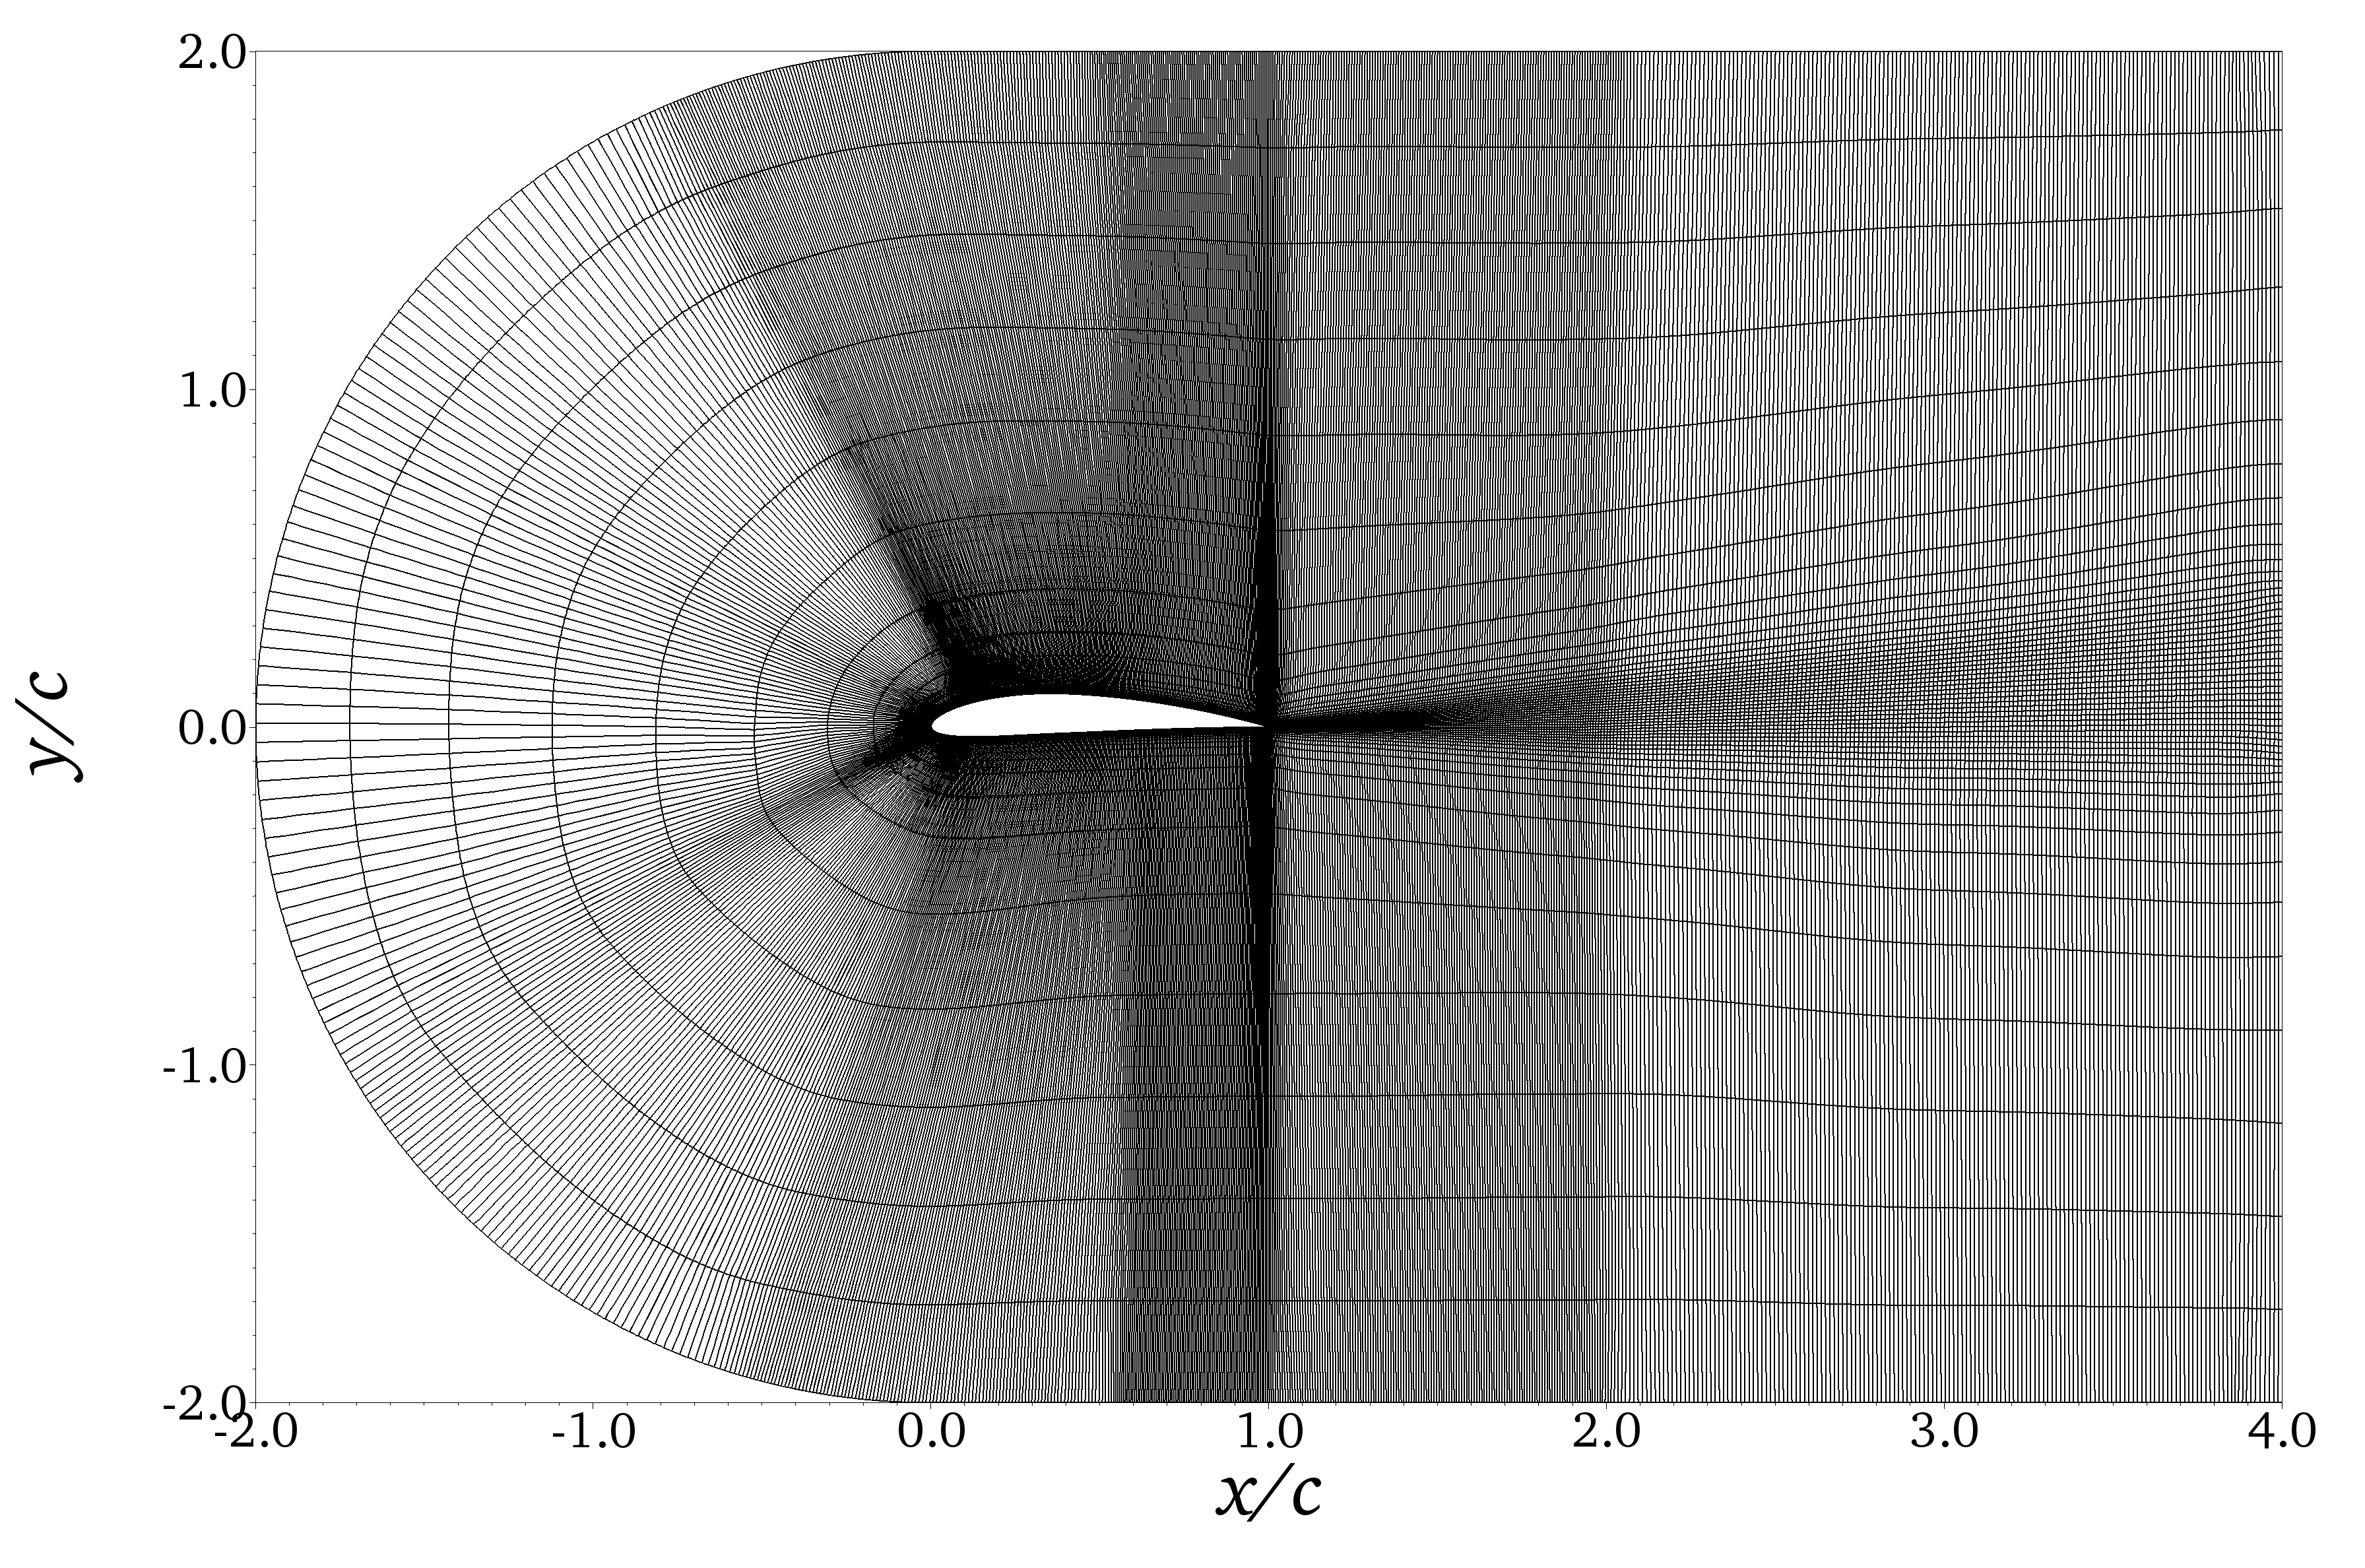
\includegraphics[width=0.46\textwidth]{wing_mesh}
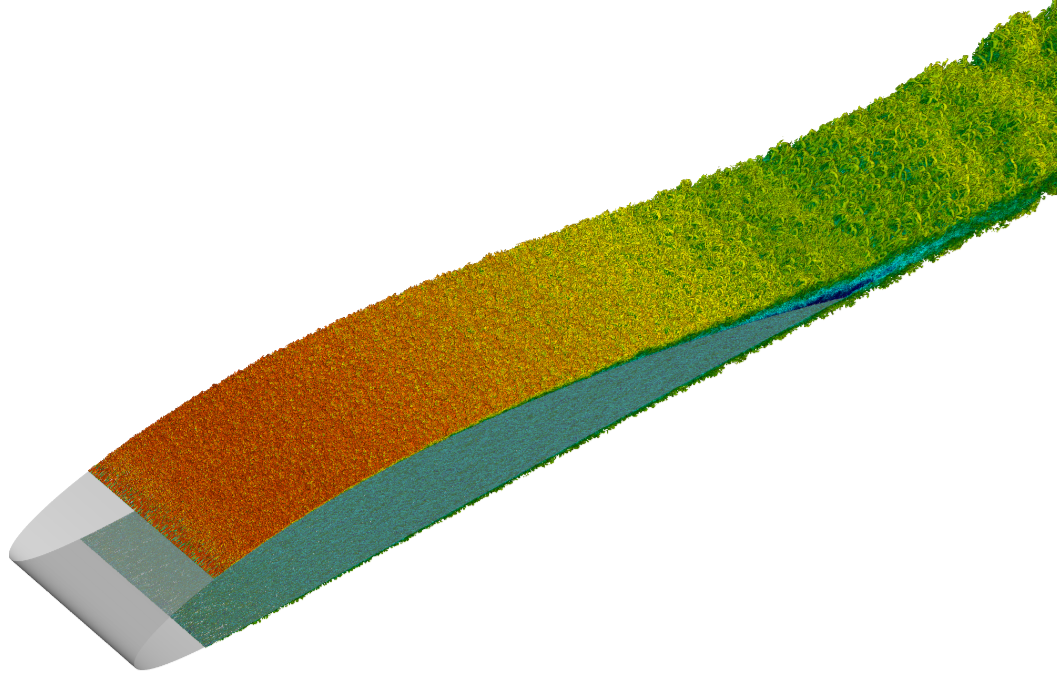
\includegraphics[width=0.46\textwidth]{wing_visualization}
\caption{(Left) Two-dimensional slice of the computational domain showing the spectral-element distribution, but not the individual GLL points. (Right) Instantaneous flow field showing coherent structures identified with the $\lambda_{2}$ method \citep{jeong_hussain}, and colored with horizontal velocity. In this figure, dark blue represents a horizontal velocity of $-0.1$ and dark red a value of $2$.}
\label{flow_field}
\end{figure}

\section{Results and discussion} 
  
As discussed in the introduction, the aim of the current study is to investigate the Reynolds-number effects on APG TBLs subjected to the same $\beta(x)$ distribution. In particular, we aim at assessing such effects on the turbulent boundary layer developing on the suction side (denoted as $ss$) of a NACA4412 wing section with $5^{\circ}$ angle of attack. To this end, we compare the results from the DNS database at $Re_{c}=400,000$ by \cite{hosseini_et_al} with the current well-resolved LES at $Re_{c}=1,000,000$. The turbulence statistics presented in this study for the $Re_{c}=1,000,000$ case were obtained after averaging for one flow-over time (where the time is non-nondimensionalized in terms of $U_{\infty}$ and $c$). Note that the spanwise width of the current simulation is twice as large as the one considered by \cite{hosseini_et_al}, a fact that effectively increases the statistical samples by a factor of two. Although this averaging period does not allow to obtain converged turbulent kinetic energy (TKE) budgets, the mean and fluctuating profiles discussed here start to exhibit convergence up to $x_{ss} /c \simeq 0.7$. The boundary-layer development, mean velocity and Reynolds-stress profiles are discussed in the next sections.

\subsection{Boundary-layer development}

In Figure \ref{beta_Reth_Ret} (top) we show the streamwise evolution of the Clauer pressure-gradient parameter $\beta$ for the TBLs on the suction side of the two wing cases under study. As expected, the two boundary layers are subjected to almost identical $\beta(x)$ distributions, with small relative differences only arising beyond $x_{ss}/c > 0.9$. Note that the boundary layers are subjected to conditions close to zero pressure gradient (ZPG) up to $x_{ss}/c \simeq 0.3$, point after which the value of $\beta$ increases beyond 0.1. In the next section we will study the velocity profiles at $x_{ss}/c=0.4$ and 0.7, in which the pressure-gradient magnitude is moderate ($\beta \simeq 0.6$) and strong ($\beta \simeq 2$), respectively. Although the value of $\beta$ increases throughout the whole suction side of the wing, an inflection point is observed at $x_{ss}/c=0.4$, which is the point of maximum camber in the NACA4412 airfoil. Beyond this point, the rate of change of $\beta$ increases significantly with $x$, a fact that is explained by the progressive reduction in airfoil thickness, which produces a larger increase in streamwise adverse pressure gradient.

In Figure \ref{beta_Reth_Ret} (middle) and (bottom) we show the streamwise evolution of the Reynolds number based on momentum thickness $Re_{\theta}$, and the friction Reynolds number $Re_{\tau}=\delta_{99} u_{\tau} / \nu$, respectively. Note that $\delta_{99}$ is the $99\%$ boundary-layer thickness, which was determined following the method described by \cite{vinuesa_diagnostic} for pressure-gradient TBLs. The $Re_{\theta}$ trends increase monotonically in the two boundary layers, due to the fact that both Reynolds number and APG promote the increase of the boundary-layer thickness. In particular, the thickenning experienced by the TBLs due to the APG significantly increases $Re_{\theta}$ in both cases, up to a maximum value of $2,800$ in the $Re_{c}=400,000$ case, and up to $Re_{\theta}=6,000$ in the higher-$Re_{c}$ wing, both observed close to the trailing edge. Regarding the friction Reynolds number, note that in the two boundary-layer cases the maximum is located at $x_{ss} / c\simeq 0.8$, and not close to the trailing edge as in $Re_{\theta}$. This is due to the fact that, although the APG increases the boundary-layer thickness, it also decreases the wall-shear stress; thus, the very strong APGs beyond $x_{ss} /c \simeq 0.8$ (where $\beta \simeq 4.1$ in both cases) produce a larger reduction in $u_{\tau}$ than the increase in $\delta_{99}$. The maximum $Re_{\tau}$ values are $373$ and $707$ in the $Re_{c}=400,000$ and $1,000,000$ wings, respectively.
\begin{figure}[t]
\centering
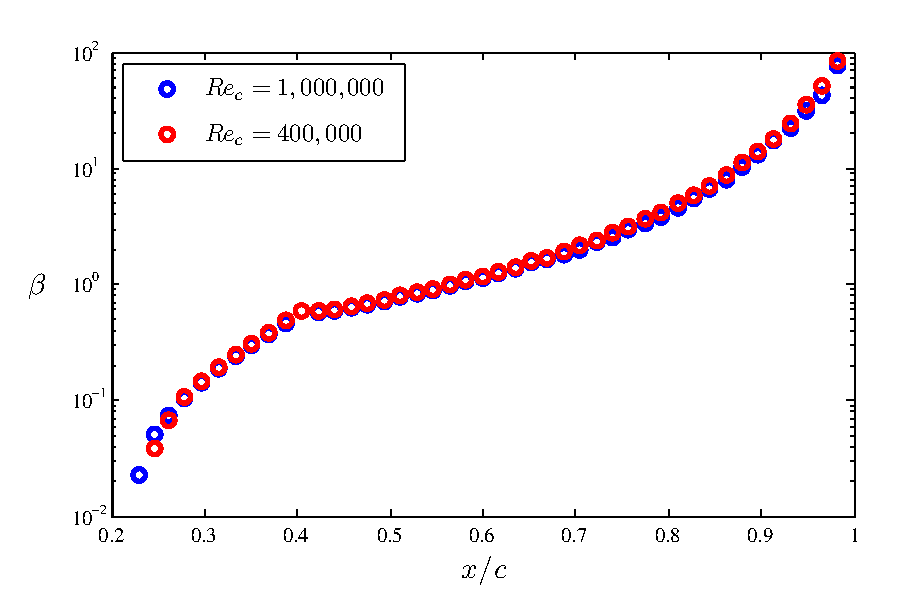
\includegraphics[width=0.49\textwidth]{beta_vs_x}
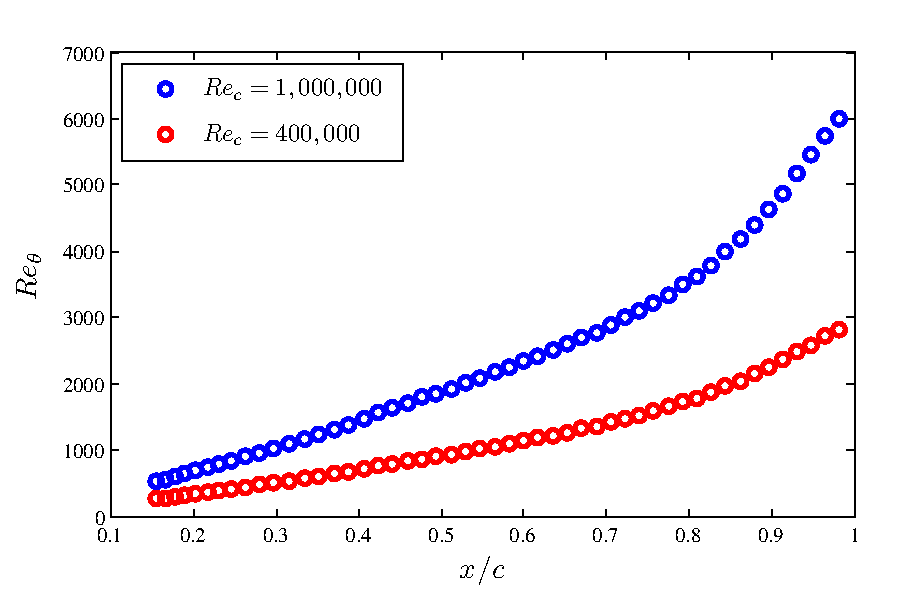
\includegraphics[width=0.49\textwidth]{Reth_vs_x}
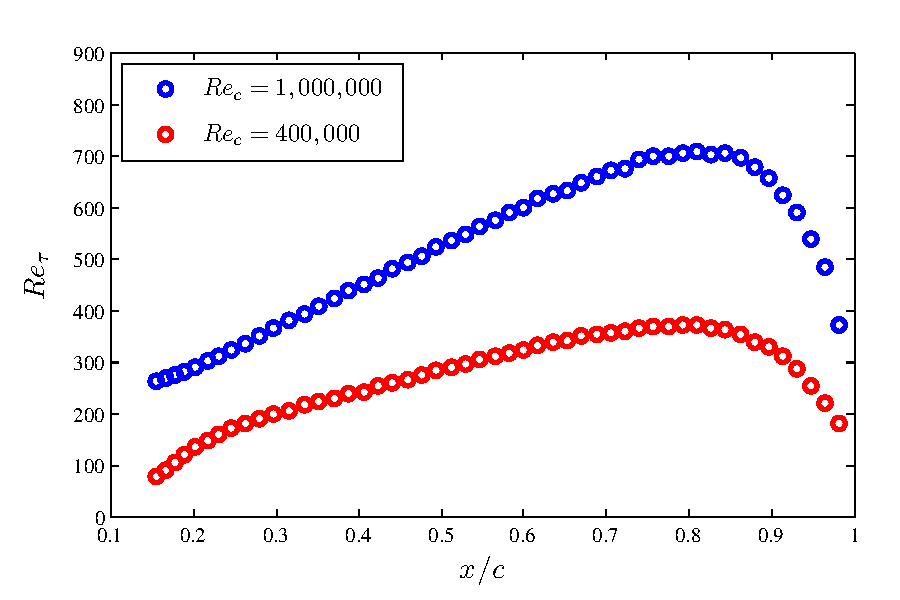
\includegraphics[width=0.49\textwidth]{Ret_vs_x}
\caption{Streamwise evolution of (top left) the Clauser pressure-gradient parameter $\beta$, (top right) the Reynolds number based on momentum thickness $Re_{\theta}$ and (bottom) the friction Reynolds number $Re_{\tau}$, for the two wing cases under study.}
\label{beta_Reth_Ret}
\end{figure}

The skin-friction coefficient $C_{f}= 2 \left (u_{\tau} / U_{e} \right )^{2}$ (where $U_{e}$ is the velocity at the boundary-layer edge) and the shape factor $H=\delta^{*} / \theta$ are shown, as a function of the streamwise position on the suction side of the wing, in Figure \ref{Cf_H}. The $C_{f}$ curves show different trends up to $x_{ss}/c \simeq 0.2$, a fact that is explained by the volume-force tripping at $x_{ss}/c=0.1$. In the present high-$Re$ case, the tripping parameters were chosen following the work by \cite{schlatter_orlu12} in ZPG TBLs; however, in the $Re_{c}=400,000$ wing the number of modes in the spanwise direction was larger than in \cite{schlatter_orlu12}, a fact that produces a long intermittent region in the post-transitional region. Nevertheless, the boundary layers can be considered to be essentially independent of the tripping beyond $x_{ss} / c \simeq 0.2$ \citep{vinuesa_diagnostic}. It can be observed that the $C_{f}$ curve in the high-$Re$ wing is below the one of the lower-$Re$ case up to $x_{ss}/c \simeq 0.9$, point after which the differences between both curves are significantly reduced. Since the two boundary layers are subjected to the same $\beta(x)$ distribution, it can be argued that the differences between both curves are due to Reynolds-number effects, a fact that is consistent with what is observed in ZPG TBLs since $C_{f}$ decreases with $Re$. Interestingly, the effect of Reynolds number becomes essentially negligible beyond $x_{ss}/c \simeq 0.9$, where the very strong APG conditions (with a value of $\beta \simeq 14$ at $x_{ss}/c=0.9$) define the state of the boundary layer. Regarding the shape factor, note that APG and Reynolds number have opposite effects on a TBL: whereas the former increases $H$ (due to the thickening of the boundary layer caused by the increased wall-normal momentum), the latter decreases the shape factor. This can also be observed in Figure \ref{Cf_H} (bottom), where the $H$ curve from the $Re_{c}=1,000,000$ is below the one from the $Re_{c}=400,000$ throughout the whole suction side of the wing. Note that, since the two boundary layers are subjected to essentially the same pressure-gradient effects, the lower values of $H$ are produced by the higher Reynolds number. The differences between the effects of $\beta$ and $Re$ on TBLs are further discussed in the next section.
\begin{figure}[t]
\centering
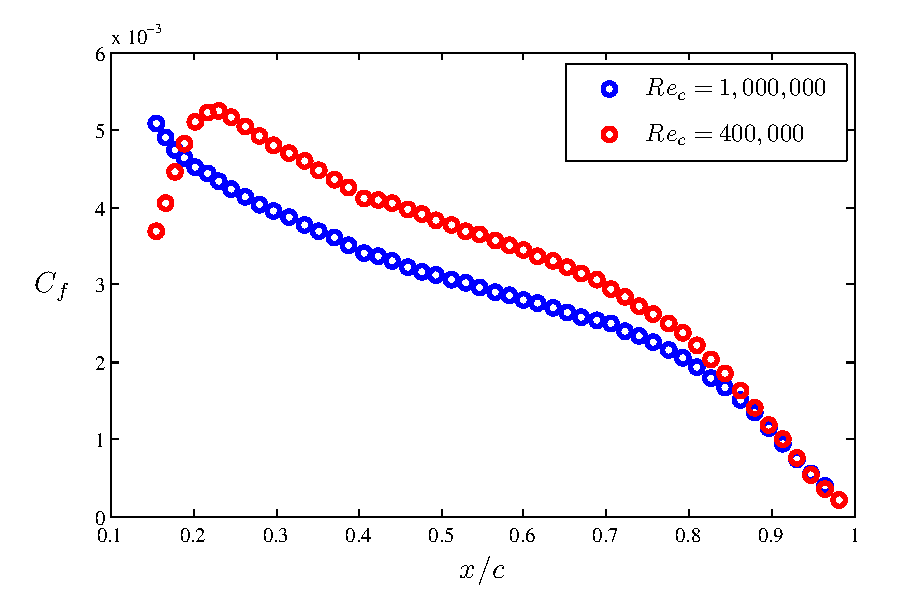
\includegraphics[width=0.49\textwidth]{Cf_vs_x}
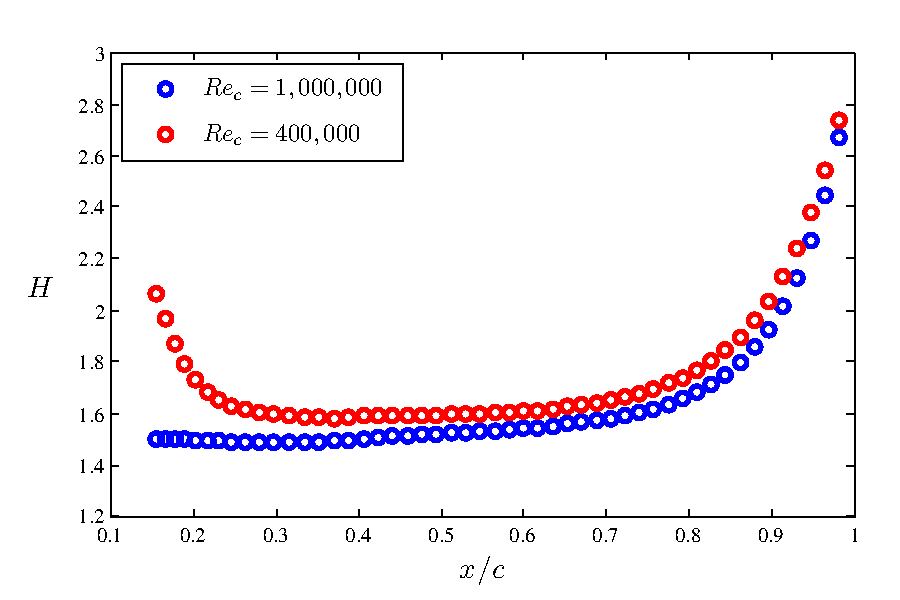
\includegraphics[width=0.49\textwidth]{H_vs_x}
\caption{Streamwise evolution of (left) the skin-friction coefficient $C_{f}$ and (right) the shape factor $H$, for the two wing cases under study.}
\label{Cf_H}
\end{figure}

\subsection{Inner-scaled mean velocity and Reynolds-stress profiles}

Figure \ref{Up_vs_yp} shows the inner-scaled mean velocity profiles at $x_{ss} /c =0.4$ and $0.7$ for the wing cases, where in the former the value of $\beta$ is around $0.6$ and in the latter $\beta \simeq 2$. Note that $U^{+}_{t}$ is the inner-scaled mean velocity in the direction tangential to the wing surface, whereas $y^{+}_{n}$ is the inner-scaled wall-normal coordinate. In Figure \ref{Up_vs_yp} (top) we show the two wing profiles, with $Re_{\tau}=242$ and $449$, together with ZPG TBL profiles at matched $Re_{\tau}$ obtained from the DNS database by \cite{schlatter_orlu10}. These comparisons are aimed at assessing the effect of the APG with respect to the baseline ZPG case, and although this comparison can be done by matching several quantities (such as $Re_{\delta^{*}}$ or $Re_{\theta}$), in the present work we fixed $Re_{\tau}$ as in the studies by \cite{monty_et_al}, \cite{harun_et_al} or \cite{bobke_et_al}. Note that by fixing $Re_{\tau}$ we compare two boundary layers which essentially exhibit the same range of spatial scales, but subjected to different pressure-gradient conditions. The first noticeable conclusion is the more prominent wakes present in the APG TBLs compared with the corresponding ZPG TBLs at the same $Re_{\tau}$, which is due to the lower skin-friction coefficient caused by the boundary-layer thickenning due to the APG. A first step towards characterizing the effect of $Re$ in the TBLs subjected to this particular $\beta(x)$ distribution is to observe the evolution of $U^{+}_{e}$ between $Re_{\tau}=242$ and $449$ in the ZPG and in the APG cases: in the former, the increase in the inner-scaled edge velocity is $11\%$, whereas in the latter it is $9.7\%$. On the other hand, the decrease in $H$ is $3.1\%$ in the ZPG boundary layers, whereas the APG cases experience a larger decrease in shape factor of $5.9\%$. These observations are also present in the profiles at $x_{ss}/c=0.7$ shown in Figure \ref{Up_vs_yp} (bottom), where the $Re_{\tau}$ values are $356$ and $671$ in the $Re_{c}=400,000$ and $1,000,000$ wing cases, respectively. At this location, the increase in $U^{+}_{e}$ is around $9.7\%$ in the ZPG boundary layer, whereas in the APG case this increase is $8.8\%$. Moreover, the shape factor decreases by $2.5\%$ from $Re_{\tau}=356$ to $671$ in the ZPG boundary layer, whereas the wings exhibit a larger decrease of $4.5\%$. On the one hand, the shape factor is larger in APG TBLs, and decreases with Reynolds number as in ZPGs (which are PG TBLs with $\beta=0$). Interestingly, the decrease in the APG case is more pronounced than the one observed in ZPG boundary layers, a fact that suggests that the values of $H$ in the low-$Re$ boundary layer are more severely affected by the APG than the ones at higher Reynolds numbers. On the other hand, the values of the inner-scaled edge velocity increase both with Reynolds number and with the APG, since in both cases the boundary layer grows and experiences a reduction in the velocity gradient at the wall. The fact that the increase in $U^{+}_{e}$ is larger in the ZPG case than in the APG indicates that in the low-Reynolds-number case the boundary layer experienced a stronger effect of the pressure gradient, therefore exhibiting a larger value of $U^{+}_{e}$ which led to a lower increase than in the $\beta=0$ case. Thus, the evolution of $U^{+}_{e}$ and $H$ indicates that the low-$Re$ boundary layer is more sensitive to the effect of the pressure gradient than the high-$Re$, when both boundary layers were subjected to the same $\beta(x)$ distribution. Additional support for this claim can be found in the mean velocity profiles at $y^{+}_{n} \simeq 25$, where the ZPG cases and the high-$Re$ wing exhibit almost identical values of the inner-scaled velocity $U^{+}_{t}$, but the low-$Re$ wing shows values below these in the two streamwise positions. Lower velocities in the buffer layer with respect to the ZPG are associated with strong effects of the APG, as documented for instance by \cite{spalart_watmuff} or \cite{bobke_et_al}. Since these lower velocities are significant in the $Re_{c}=400,000$ wing, it can be stated that the effect of the APG is more pronounced in this case than in the high-$Re$ wing.
\begin{figure}[t]
\centering
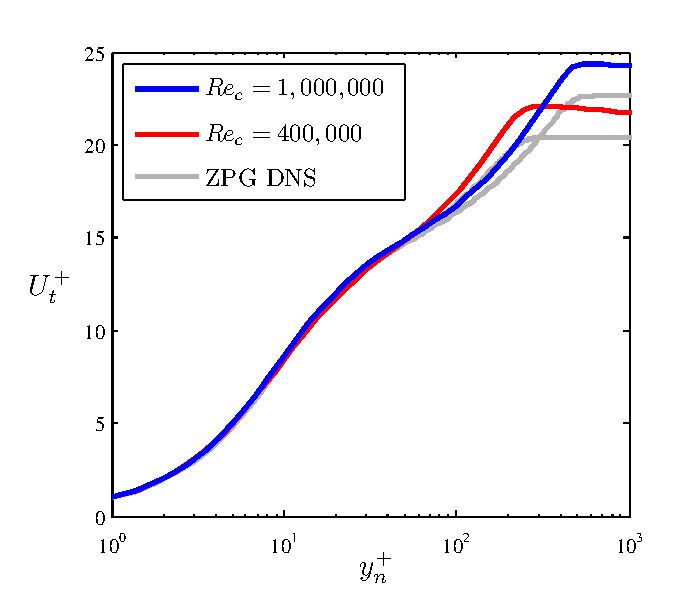
\includegraphics[width=0.49\textwidth]{Up_vs_yp_04}
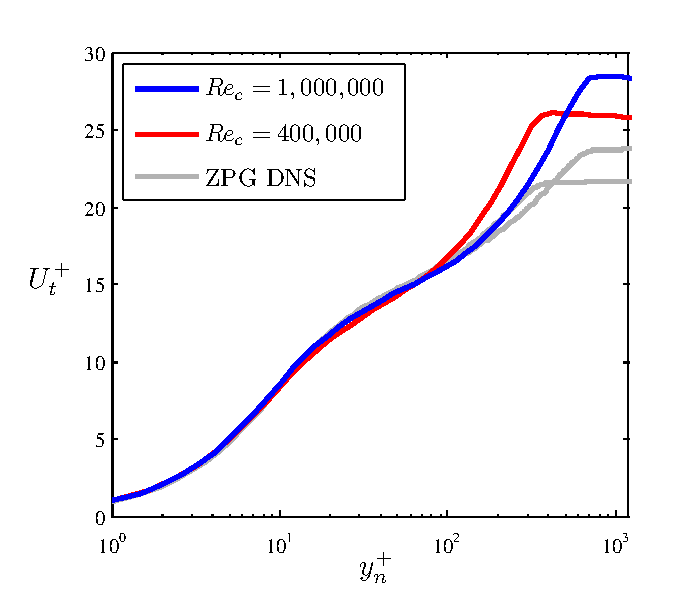
\includegraphics[width=0.49\textwidth]{Up_vs_yp_07}
\caption{Inner-scaled mean velocity profiles at (left) $x_{ss}/c=0.4$ and (right) $x_{ss}/c=0.7$ for the two wing cases under study, compared with the DNS results of ZPG TBL by \cite{schlatter_orlu10} at matched $Re_{\tau}$ values.}
\label{Up_vs_yp}
\end{figure}

As discussed by \cite{harun_et_al} or \cite{bobke_et_al}, the APG energizes the outer region of the boundary layer, producing more energetic turbulent structures. This effect is also observed when increasing the Reynolds number in a ZPG TBL, since as the boundary layer develops the outer region exhibits more energetic structures as shown for instance in the experiments by \cite{hutchins_marusic} and the numerical simulations by \cite{eitel_amor_et_al}. However, the mean velocity profiles shown in Figure \ref{Up_vs_yp} suggest that there may be differences in the way that this energizing process takes place, since the the evolution of the mean flow parameters with Reynolds number is not the same in the $\beta=0$ (ZPG) as in the APG cases. In particular, it is interesting to note that at low Reynolds numbers the effect of the APG appears to be more prominent than at higher $Re$. Large-scale energetic motions develop in ZPG TBLs at increasing Reynolds number together with the development of the outer region of the boundary layer. The present results suggest that such development of the outer region takes place in a different way when an APG is present, a fact that is closely connected to the much larger wall-normal convection in APGs. In APG TBLs there are two complementing mechanisms responsible for the development of the boundary-layer outer region, namely due to $\beta$ and due to $Re$. In order to further analyze the differences between these mechanisms, several components of the Reynolds-stress tensor are shown for the two wing cases at $x_{ss}/c=0.4$ and $0.7$ in Figure \ref{uup_vs_yp}. Note that we also show the inner-scaled streamwise velocity fluctuation profiles from the ZPG DNS by \cite{schlatter_orlu10} at matched $Re_{\tau}$ values for comparison. The first important conclusion that can be drawn from Figure \ref{uup_vs_yp} is the fact that all the components of the Reynolds-stress tensor exhibit a more energetic outer region in comparison with ZPG TBLs, as discussed for instance by \cite{kitsios_et_al} or \cite{bobke_et_al}. Moreover, in Figure \ref{uup_vs_yp} (top) it can be observed that the increase in the near-wall peak of the tangential velocity fluctuation profile $\overline{u^{2}_{t}}^{+}$ from $Re_{\tau}=242$ to $449$ is of around $4.5\%$, which interestingly is approximately the same increase as in the wing cases. In fact, and as discussed by \cite{eitel_amor_et_al}, the wall-resolved LES method employed in the present study slightly attenuates the near-wall peak of $\overline{u^{2}_{t}}^{+}$, a fact that would indicate that the increase in the wing boundary layers is slightly larger than in the ZPG. On the other hand, the $Re_{c}=400,000$ wing exhibits a much more energetic outer region than the corresponding ZPG case at the same $Re_{\tau}$: for instance, at $y^{+}_{n} = 100$ the low-$Re$ wing case shows a $\overline{u^{2}_{t}}^{+}$ value $41\%$ larger than the ZPG at the same location. On the other hand, this difference is significantly lower in the high-$Re$ wing, where the $\overline{u^{2}_{t}}^{+}$ is only around $17\%$ higher than the ZPG at $y^{+}_{n}=200$ (note that this wall-normal location corresponds to $y_{n}/\delta_{99} \simeq 0.29$, {\it i.e.}, approximately the same distance from the wall in outer units as in the low-$Re$ case). This suggests that in the low-$Re$ APG there is a higher energy concentration in the outer region than in the high-$Re$ one. This is further confirmed by the results shown in Figure \ref{uup_vs_yp} (bottom) at $x_{ss}/c=0.7$, where the $Re_{\tau}$ values are 356 and 671. Firstly, the increase in the near-wall peak of $\overline{u^{2}_{t}}^{+}$ is slightly larger in the APG boundary layers ($5.1\%$) than in the ZPG ($4.5\%$), a difference that could be larger if the fact that the well-resolved LES slightly attenuates the near-wall peak in the high-$Re$ case. However, the most significant result in Figure \ref{uup_vs_yp} (bottom) is the fact that both APG boundary layers exhibit a plateau in the outer region of the tangential velocity fluctuation profile. In particular, the $\overline{u^{2}_{t}}^{+}$ value in this plateau is larger in the lower-$Re$ wing ($5.75$) than in the high-$Re$ case ($5.0$). Since the high-$Re$ wing exhibits a larger value of the near-wall peak, the ratio between this maximum and the plateau in the outer region is significantly larger in the $Re_{c}=1,000,000$ case ($1.78$) than in the $Re_{c}=400,00$ wing ($1.48$). This is a very relevant result, since it shows not only that the energizing mechanisms of the outer region in the boundary layer are different when they are connected to APG than when they are associated to $Re$, but also that lower-$Re$ TBLs are more sensitive to pressure-gradient effects than high-$Re$ ones. In particular, the tangential velocity fluctuation profiles show larger values in the outer region in the lower-$Re$ case, which is a manifestation of more prominent energy accumulation in the large-scale motions than in the high-$Re$ APG boundary layer.
\begin{figure}[t]
\centering
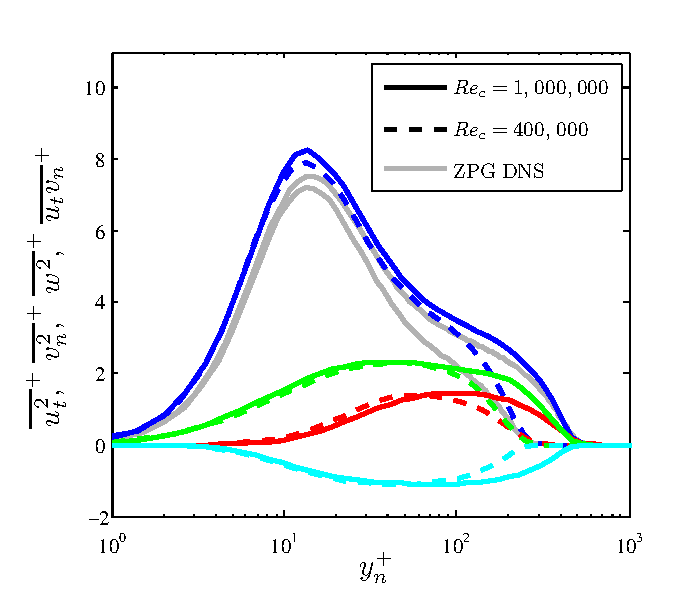
\includegraphics[width=0.49\textwidth]{uup_vs_yp_04}
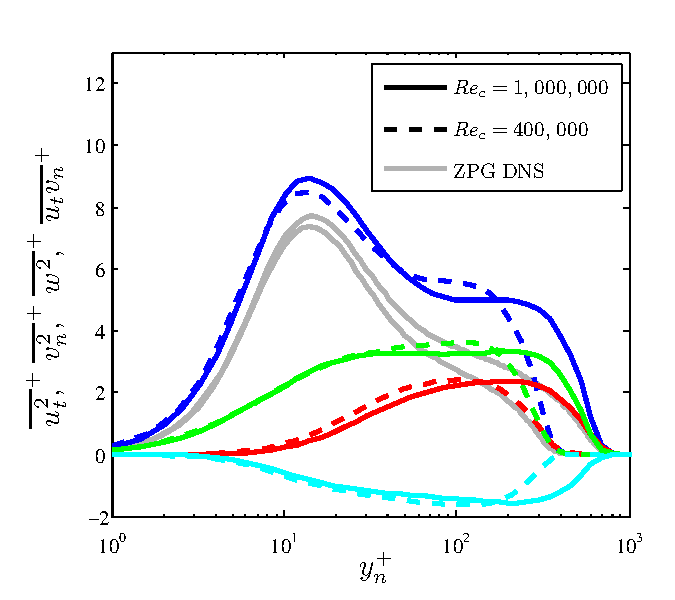
\includegraphics[width=0.49\textwidth]{uup_vs_yp_07}
\caption{Selected components of the inner-scaled Reynolds-stress tensor at (left) $x_{ss}/c=0.4$ and (right) $x_{ss}/c=0.7$ for the two wing cases under study, compared with the DNS results of ZPG TBL by \cite{schlatter_orlu10} at matched $Re_{\tau}$ values. The Reynolds stresses are represented as: {\color{blue}\solid} tangential {\color{red}\solid} wall-normal and {\color{green}\solid} spanwise velocity fluctuations, and {\color{cyan}\solid} Reynolds shear stress.}
\label{uup_vs_yp}
\end{figure}

\section{Summary and conclusions}

The present study is aimed at further understanding the mechanisms responsible for the development of the outer region of TBLs and for the energizing of the large-scale motions, as well as their connection with APGs and increasing Reynolds number. To this end, we performed a well-resolved LES of the flow around a NACA4412 wing section at $Re_{c}=1,000,000$, with $5^{\circ}$ angle of attack, using the spectral-element code Nek5000. The setup is similar to the one employed by \cite{hosseini_et_al} to perform a DNS of the same flow case at a lower $Re_{c}=400,000$. The boundary layers developing on the suction side of the two wing sections are subjected to essentially the same streamwise Clauser pressure-gradient distribution $\beta(x)$, a fact that allows to characterize the effect of the Reynolds number in APG TBLs subjected to an increasing APG magnitude. 

As a TBL develops, the increasing Reynolds number produces a more energetic outer region, a fact that is manifested in the Reynolds-stress tensor profiles. On the other hand, an APG also produces more energetic large-scale motions in the outer region of the boundary layer due to the lift-up effect and the increased wall-normal convection associated to it. Our results indicate that the skin-friction curve from the wing at $Re_{c}=1,000,000$ is below the one at $Re_{c}=400,000$ (up to around $x_{ss}/c \simeq 0.9$), a fact that is consistent with the well-known effect of Reynolds number in ZPG TBLs. Moreover, the shape factor curve in the high-$Re$ wing is also below the one at $Re_{c}=400,000$, which is associated with another effect of Reynolds number, {\it i.e.}, to reduce $H$. 

We also analyzed the inner-scaled mean velocity profiles at $x_{ss}/c=0.4$ and $0.7$, which are subjected to $\beta$ values of $0.6$ and $2$, respectively. At $x_{ss}/c=0.4$, the increase of $U^{+}_{e}$ from $Re_{\tau}=242$ to $449$ is $9.7\%$, which is lower than the increase in ZPG TBLs over the same $Re_{\tau}$ range ($11\%$). Similarly, at $x_{ss}/c=0.7$ the increase in $U^{+}_{e}$ from $Re_{\tau}=356$ to $671$ is $8.8\%$, also below the one in ZPGs, which is $9.7\%$. On the other hand, the shape factor is reduced at $x_{ss}/c=0.4$ by $5.9\%$ and at $x_{ss}/c=0.7$ by $4.5\%$ (compared to only $3.1\%$ and $2.5\%$ in the corresponding ZPG case). The steeper decrease in $H$ and the more moderate increase in $U^{+}_{e}$ compared to ZPG TBLs indicate that the lower-$Re$ APG is more sensitive to pressure-gradient effects than the high-$Re$ one. This conclusion is supported by the observations on several components of the Reynolds-stress tensor, in particular in the tangential velocity fluctuation profile. Our results show that at $x_{ss}/c=0.4$ the lower-$Re$ wing exhibits a larger ratio of $\overline{u^{2}_{t}}^{+}$ in the outer region with respect to the corresponding ZPG case than the high-$Re$ case, again indicating a more pronounced effect of the APG on the lower Reynolds number wing. Regarding the profiles at $x_{ss}/c=0.7$, it is interesting to note that although the high-$Re$ wing exhibits a larger near-wall peak in $\overline{u^{2}_{t}}^{+}$ than the lower-$Re$ case, the latter exhibits larger values in the outer region. Thus, while the former shows a value of $5.0$ in the plateau located in the outer part of the $\overline{u^{2}_{t}}^{+}$ profile, the latter exhibits a higher value of $5.75$. Consequently, the ratio between the near-wall peak and the plateau in the $\overline{u^{2}_{t}}^{+}$ profile is $1.78$ in the high-$Re$ wing, and $1.48$ in the lower-$Re$ case. This shows that the energy distribution in the two wing boundary layers, subjected to the same $\beta(x)$, is significantly different. Further analysis of these results will help to elucidate the differences in the mechanisms for outer-region energizing due to APG and Reynolds number. 

\section{Acknowledgments}

The simulations were performed on resources provided by the Swedish National Infrastructure for Computing (SNIC) at the Center for Parallel Computers (PDC), in KTH, Stockholm. RV and PS acknowledge the funding provided by the Swedish Research Council (VR) and from the Knut and Alice Wallenberg Foundation. This research is also supported by the ERC Grant No. ``2015-AdG-694452, TRANSEP'' to DH.

\section{References}

%% The Appendices part is started with the command \appendix;
%% appendix sections are then done as normal sections
%% \appendix

%% \section{}
%% \label{}

%% If you have bibdatabase file and want bibtex to generate the
%% bibitems, please use
%%
%\bibliographystyle{elsarticle-harv} 
%\bibliography{wing_bib}
%%  \bibliography{<your bibdatabase>}

%% else use the following coding to input the bibitems directly in the
%% TeX file.

%\begin{thebibliography}{00}
%
%%% \bibitem[Author(year)]{label}
%%% Text of bibliographic item
%
%\bibitem[ ()]{}
%
%\end{thebibliography}
%\end{document}

%\endinput
%%
%% End of file `elsarticle-template-harv.tex'.
